% Retoca las líneas marcadas con TODO según las necesidades

\documentclass[oneside,a4paper,12pt]{book} % TODO: cambia "oneside" por "twoside" a la hora de imprimirlo

\usepackage[spanish]{babel}
\usepackage[utf8]{inputenc}
\usepackage{geometry}
\usepackage{makeidx}
\usepackage{url}
\usepackage{graphicx}
\usepackage{color}
\usepackage{caption}
\usepackage{acronym}
\usepackage{hyphenat}
\usepackage{a4wide}
\usepackage[normalsize]{subfigure}
\usepackage{float}
\usepackage{titlesec}
\usepackage[export]{adjustbox}
\usepackage[Lenny]{fncychap}
\usepackage{listings} % para poder hacer uso de "listings" propios (p.ej. códigos)
\usepackage{eurosym} % para poder usar el símbolo del euro con \euro {xx}
\usepackage{hyperref} % TODO: añade la opción hidelinks para imprimirlo (los enlaces no aparecerán resaltados)

% Para que no parta las palabras
\pretolerance=10000

\newcommand{\bigrule}{\titlerule[0.5mm]} \titleformat{\chapter}[display] % cambiamos el formato de los capítulos
{\bfseries\Huge} % por defecto se usaron caracteres de tamaño huge en negrita
{% contenido de la etiqueta 
\titlerule % línea horizontal 
\filright % texto alineado a la derecha 
\Large\chaptertitlename\ % capítulo e índice en tamaño large
\Large % en lugar de 
\Huge \Large\thechapter} 
{0mm} % espacio mínimo entre etiqueta y cuerpo
{\filright} % texto del cuerpo alineado a la derecha
[\vspace{0.5mm} \bigrule] % después del cuerpo, dejar espacio vertical y trazar línea horizontal gruesa
\geometry{a4paper, left=3.5cm, right=2cm, top=3cm, bottom=2cm, headsep=1.5cm}

% Estilos para ilustrar códigos:
\definecolor{code_green}{rgb}{0,0.6,0}
\definecolor{code_gray}{rgb}{0.5,0.5,0.5}
\definecolor{code_mauve}{rgb}{0.58,0,0.82}

\lstset{frame=tb,
  language=C,
  aboveskip=3mm,
  belowskip=3mm,
  showstringspaces=false,
  columns=flexible,
  basicstyle={\small\ttfamily},
  numbers=none,
  numberstyle=\tiny\color{code_gray},
  keywordstyle=\color{blue},
  commentstyle=\color{code_green},
  stringstyle=\color{code_mauve},
  breaklines=true,
  breakatwhitespace=true,
  tabsize=3
}

\lstset{frame=tb,
  language=C++,
  aboveskip=3mm,
  belowskip=3mm,
  showstringspaces=false,
  columns=flexible,
  basicstyle={\small\ttfamily},
  numbers=none,
  numberstyle=\tiny\color{code_gray},
  keywordstyle=\color{blue},
  commentstyle=\color{code_green},
  stringstyle=\color{code_mauve},
  breaklines=true,
  breakatwhitespace=true,
  tabsize=3
}

\lstset{frame=tb,
  language=Python,
  aboveskip=3mm,
  belowskip=3mm,
  showstringspaces=false,
  columns=flexible,
  basicstyle={\small\ttfamily},
  numbers=none,
  numberstyle=\tiny\color{code_gray},
  keywordstyle=\color{blue},
  commentstyle=\color{code_green},
  stringstyle=\color{code_mauve},
  breaklines=true,
  breakatwhitespace=true,
  tabsize=3
}

% Definición de mis propios tipos: Códigos, Ecuaciones y Tablas
\DeclareCaptionType{code}[Código][Listado de códigos]
\DeclareCaptionType{myequation}[Ecuación][Listado de ecuaciones]

% TODO: especifica las reglas de separación que consideres. Algunos ejemplos:
\hyphenation{fuer-tes}
\hyphenation{mul-ti-ca-pa}
\hyphenation{res-pues-ta}
\hyphenation{di-fe-ren-tes}
\hyphenation{de-sa-rro-lla-dos}
\hyphenation{re-pre-sen-tan-do}

 % archivo de configuraci�n de estilo

\makeindex

\begin{document}
\baselineskip 1.35\baselineskip

\frontmatter

\thispagestyle{empty}
\vspace{2cm}

\begin{figure}[htb]
  \centerline{\resizebox{.45\textwidth}{!}{
\includegraphics{figs/logo_urjc}}}
\end{figure}

\begin{center}
  \vspace{5mm}
    {\Large {ESCUELA DE INGENIERÍA DE FUENLABRADA}}
  \vspace{1cm}
  
  {\Large {GRADO EN INGENIERÍA DE ROBÓTICA SOFTWARE}}
  \vspace{20mm}

   {\Large {\textbf{TRABAJO FIN DE GRADO}}}


   \vspace{2cm}

  {\large \textbf{Diseño de controladores gamificados\\
               para rotot de rehabilitación }}

  \vspace{2cm}
  
  {\bf Autor/a}: Sofía Perales Díez
  
  {\bf Tutor}: Julio S. Lora Millán 
  
  {\bf Co-Tutor}: Juan A. Castaño Peña \\

\vspace{3cm}

  Curso académico 2024 / 2025

 
\end{center}

\clearpage
\thispagestyle{empty}


% Este diseño se corresponde con la licencia CC-BY-NC-SA.
% Por supuesto, puedes poner la licencia que mejor se adapte al propósito de tu trabajo.
% Recuerda que, si no se especifica ninguna licencia, esta -como cualquier creación artística- pasaría a estar licenciada con todos los derechos reservados (copyright).

\cleardoublepage

\begin{flushright}
\begin{figure}
 \ \ \ \ 
\includegraphics[width=0.25\linewidth,right]{figs/by-sa.png}
 \label{fig:cc} 
 \end{figure}
\end{flushright}

\

\

\

\noindent
Este trabajo se distribuye bajo los términos de la licencia internacional \href{http://creativecommons.org/licenses/by-sa/4.0/}{CC BY-SA International License} (Creative Commons Attribution-ShareAlike 4.0). Usted es libre de \textit{(a) compartir}: copiar y redistribuir el material en cualquier medio o formato para cualquier propósito, incluso comercialmente; y \textit{(b) adaptar}: remezclar, transformar y construir a partir del material para cualquier propósito, incluso comercialmente. La licenciante no puede revocar estas libertades en tanto usted siga los términos de la licencia:

\begin{itemize}
\item \textit{Atribución}. Usted debe dar \href{https://creativecommons.org/licenses/by-sa/4.0/deed.es#ref-appropriate-credit}{crédito de manera adecuada}, brindar un enlace a la licencia, e indicar \href{https://creativecommons.org/licenses/by-sa/4.0/deed.es#ref-indicate-changes}{si se han realizado cambios}. Puede hacerlo en cualquier forma razonable, pero no de forma tal que sugiera que usted o su uso tienen el apoyo de la licenciante.
\item \textit{Compartir igual}. Si remezcla, transforma o crea a partir del material, debe distribuir su contribución bajo la \href{https://creativecommons.org/licenses/by-sa/4.0/deed.es#ref-same-license}{misma licencia} del original.\\
No hay restricciones adicionales — No puede aplicar términos legales ni \href{https://creativecommons.org/licenses/by-sa/4.0/deed.es#ref-technological-measures}{medidas tecnológicas} que restrinjan legalmente a otras a hacer cualquier uso permitido por la licencia.
\end{itemize}

\begin{flushright}
		\vspace{7.0 cm}
		\emph{Documento de} \textbf{Sofía Perales Díez}. % TODO: pon aquí tu nombre cuando hagas el documento
\end{flushright}



\cleardoublepage

\chapter*{Agradecimientos}

En primer lugar, me gustaría agradecer a la Universidad Rey Juan Carlos por brindarme la oportunidad de formar parte de esta institución.
A todo el equipo docente que me ha formado académicamente, y en especial, a mis tutores Julio Salvador Lora y Juan Alejandro Castaño por la confianza y el apoyo depositado en mi para llevar a cabo este proyecto.\\

Agradecer a mis padres por todo lo que me han dado y por estar siempre a mi lado apoyándome e impulsándome a superarme y convertirme en la mejor versión de mí misma. 
A mi hermana, de la que aprendo todos los días y que me motiva a ser alguien en quien pueda inspirarse y confiar. 
Y a mi abuela, que es un referente para mí y me ha defendido siempre.\\

También agradecer a mis amigos, aquellos que se alegran por mis logros como si fuesen los suyos propios. 
Por la paciencia que tienen conmigo y por estar en las buenas y en las malas. 
A Nuria de la Fuente, por ser mi alma gemela desde el primer momento que nos conocimos. 
A Lucía Álvarez, por convertirse en mi hermana, doy gracias por habernos encontrado en la otra punta del mundo.
A mis amigas del cole, quienes me han visto crecer y con las que he compartido la mayor parte de mi vida.
Y a mis amigos de la universidad, gracias por las risas, los desayunos en la cafetería y sobre todo por el apoyo en momentos de estrés.
Porque los ratitos con vosotros han hecho que el camino sea más fácil y ameno.\\

Y por último, gracias a Hispamast y todos sus empleados por darme la oportunidad de hacer las prácticas de empresa y formarme laboralmente.
En especial a mis jefes y amigos Javier Trabalón y Alejandro Caballero, por cuidarme y tomarme como vuestra aprendiz. 
Gracias a vosotros he disfrutado de cada minuto durante las prácticas y ojalá sigamos compartiendo momentos juntos.\\

Todos vosotros me habeis hecho ser quien soy, gracias desde el corazón.\\
\ % Algo de separación...

\

\

\

\

\begin{flushright}
		\vspace{4.0 cm}
		\emph{A mi yo de pequeña;\\
      quien soñaba con ser ingeniera,
	  enhorabuena lo hemos conseguido}\\
		\par
		\vspace{1.0 cm}
		Madrid, xx de xxxxxx de 2025\\ %\today
		\emph{Sofía Perales Díez}
\end{flushright}

\thispagestyle{empty}



\cleardoublepage

\chapter*{Resumen\markboth{Resumen}{Resumen}}

El ictus es una de las principales causas de discapacidad motora, afectando a la movilidad y calidad de vida de los pacientes.
La rehabilitación temprana, durante los primeros meses tras el ictus, es crucial para optimizar la recuperación funcional.\\

En los últimos años, diversos estudios han evaluado la efectividad de la integración de dispositivos robóticos en los procesos de rehabilitación, mostrando resultados prometedores en cuanto a la mejora de la movilidad y participación del paciente.\\

El presente trabajo tiene como objetivo desarrollar un sistema de rehabilitación motora para la extremidad superior de pacientes post-ictus, basado en un entorno gamificado personalizado que potencie la motivación del paciente y mejore la efectividad del tratamiento.
La plataforma consta de tres componentes principales: una interfaz de control que permite al terapeuta adaptar las sesiones de rehabilitación de acuerdo con las capacidades del paciente, una interfaz de visualización que facilita el monitoreo en tiempo real del progreso del paciente, y una interfaz de juego que permite hacer los ejercicios de rehabilitación de manera interactiva y dinámica.
Además, el sistema almacena los datos más relevantes durante la terapia, lo que facilita realizar un análisis detallado y evaluar el progreso de cada paciente.\\

Se espera que este sistema no solo facilite la rehabilitación motora, sino que también mejore la motivación y adherencia al tratamiento, ofreciendo una solución más efectiva para la recuperación post-ictus, gracias a su adaptación personalizada a las necesidades de cada paciente, un mayor control sobre los ejercicios y la escalabilidad que permite ajustarse a diferentes modos de terapia.


\cleardoublepage

\chapter*{Abstract\markboth{Abstract}{Abstract}}

Stroke is one of the main causes of motor disability, affecting patients' mobility and quality of life.
Early rehabilitation, during the first months after stroke, is crucial to optimize functional recovery.\\

In recent years, several studies have evaluated the effectiveness of integrating robotic devices in rehabilitation processes, showing promising results in terms of improved patient mobility and participation.\\

The present work aims to develop a motor rehabilitation system for the upper extremity of post-stroke patients, based on a personalized gamified environment that enhances patient motivation and improves treatment effectiveness.
The platform consists of three main components: a control interface that allows the therapist to adapt the rehabilitation sessions according to the patient's capabilities, a visualization interface that facilitates real-time monitoring of the patient's progress, and a game interface that allows the rehabilitation exercises to be performed interactively and dynamically.
In addition, the system stores the most relevant data during therapy, which facilitates detailed analysis and evaluation of each patient's progress.\\

It is expected that this system will not only facilitate motor rehabilitation, but also improve motivation and adherence to treatment, offering a more effective solution for post-stroke recovery, thanks to its personalized adaptation to the needs of each patient, greater control over the exercises and scalability that allows it to adjust to different modes of therapy.


\cleardoublepage

\chapter*{Acrónimos\markboth{Acrónimos}{Acrónimos}}

% Añade a continuación los acrónimos que uses en el documento. Algunos ejemplos:
\begin{acronym}
	\acro{API}{\emph{Interfaz de Programación de Aplicaciones}}
	\acro{ECV}{\emph{Enfermedad Cerebrovascular}}
	\acro{EPIK}{\emph{Estimulación para Promover la Independencia mediante Kinect}}
	\acro{GUI}{\emph{Interfaz Gráfica de Usuario}}
	\acro{MIDAS}{\emph{Multi-sensorial Immersive Dynamic Autonomous System}}
	\acro{OMS}{\emph{Organización Mundial de la Salud}}
	\acro{ROS}{\emph{Sistema Operativo Robótico}}
	\acro{RV}{\emph{Realidad Virtual}}
	\acro{SAFE}{\emph{Alianza Europea contra el ictus}}
	\acro{SEN}{\emph{Sociedad Española de Neurología}}
	\acro{SERMEF}{\emph{Socidad Española de Rehabilitación y Medicina Física}}
	\acro{SNS}{\emph{Sistema Nacional de Salud}}
\end{acronym}


\cleardoublepage

\tableofcontents

\listoffigures

\listofcodes

\listofmyequations

%\listoftables

%\pagestyle{empty}

\cleardoublepage

 % aqu� se cargan todas las "primeras p�ginas"

% Bibliograf�a
\let\OLDthebibliography=\thebibliography
\def\thebibliography#1{\OLDthebibliography{#1}
  \addcontentsline{toc}{chapter}{\bibname}}

\mainmatter

\setcounter{page}{1}
\chapter{Introducción}
\label{cap:capitulo1}
\setcounter{page}{1}

\begin{flushright}
\begin{minipage}[]{10cm}
\emph{Quizás algún fragmento de libro inspirador...}\\
\end{minipage}\\

Autor, \textit{Título}\\
\end{flushright}

\vspace{1cm}

Escribe aquí un párrafo explicando brevemente lo que vas a contar en este capítulo. En este primer capítulo, el de introducción, se trata de dar un contexto amplio y atractivo del trabajo. Comienza hablando de un contexto general y acaba hablando del contexto más específico en el que se enmarca el proyecto. Es el capítulo idóneo para incluir todas las referencias bibliográficas que hayan tratado este tema; suponen un fuerte respaldo al trabajo.\\

\section{La primera sección}
\label{sec:miseccion} % etiqueta para luego referenciar esta sección

En los textos puedes poner palabras en \textit{cursiva}, para aquellas expresiones en sentido \textit{figurado}, palabras como \textit{robota}, que está fuera del diccionario castellano, o bien para resaltar palabras de una colección: \textit{(a)} es la primera letra del abecedario, \textit{(b)} es la segunda, etc.\\

Al poner las dos líneas del anterior párrafo, este aparecerá separado del anterior. Si no las pongo, los párrafos aparecerán pegados. Sigue el criterio que consideres más oportuno.

\section{Segunda sección}
\label{sec:segundaseccion}

No olvides incluir imágenes y referenciarlas, como la Figura \ref{fig:roomba}.

\begin{figure} [h!]
  \begin{center}
    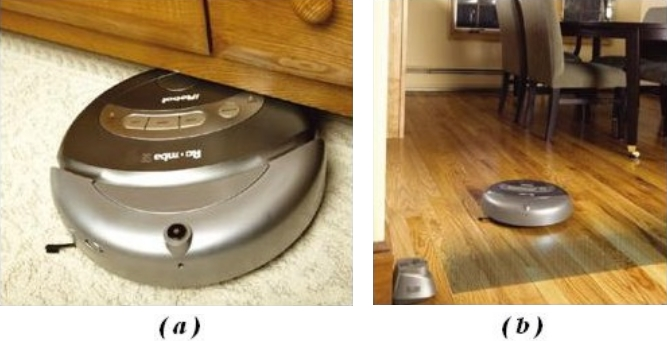
\includegraphics[width=8cm]{figs/roomba}
  \end{center}
  \caption{Robot aspirador Roomba de iRobot.}
  \label{fig:roomba}
\end{figure}\

Ni tampoco olvides de poner las URLs como notas al pie. Por ejemplo, si hablo de la Robocup\footnote{\url{http://www.robocup.org}}.

\subsection{Números}
\label{sec:subseccion}

En lugar de tener secciones interminables, como la Sección \ref{sec:miseccion}, divídelas en subsecciones.

Para hablar de números, mételos en el entorno \textit{math} de \LaTeX, por ejemplo, $1.5Kg$. También puedes usar el símbolo del Euro como aquí: 1.500\euro.

\subsection{Listas}

Cuando describas una colección, usa \texttt{itemize} para ítems o \texttt{enumerate} para enumerados. Por ejemplo:

\begin{itemize}
 \item \textit{Entorno de simulación.} Hemos usado dos entornos de simulación: uno en 3D y otro en 2D.
 \item \textit{Entornos reales.} Dentro del campus, hemos realizado experimentos en Biblioteca y en el edificio de Gestión.
\end{itemize}\

\begin{enumerate}
 \item Primer elemento de la colección.
 \item Segundo elemento de la colección.
\end{enumerate}\

\paragraph{Referencias bibliográficas}
\label{sec:referencias}

Cita, sobre todo en este capítulo, referencias bibliográficas que respalden tu argumento. Para citarlas basta con poner la instrucción \verb|\cite| con el identificador de la cita. Por ejemplo: libros como \cite{vega12e}, artículos como \cite{vega19b}, URLs como \cite{vega19a}, tesis como \cite{vega18b}, congresos como \cite{vega18a}, u otros trabajos fin de grado como \cite{vega08b}.

Las referencias, con todo su contenido, están recogidas en el fichero \texttt{bibliografia.bib}. El contenido de estas referencias está en formato \texttt{BibTex}. Este formato se puede obtener en muchas ocasiones directamente, desde plataformas como \texttt{Google Scholar} u otros repositorios de recursos científicos.

Existen numerosos estilos para reflejar una referencia bibliográfica. El estilo establecido por defecto en este documento es APA, que es uno de los estilos más comunes, pero lo puedes modificar en el archivo \texttt{memoria.tex}; concretamente, cambiando el campo \verb|apalike| a otro en la instrucción \verb|\bibliographystyle{apalike}|. 

\

\

\

Y, para terminar este capítulo, resume brevemente qué vas a contar en los siguientes.


\chapter{Objetivos}
\label{cap:capitulo2}

\begin{flushright}
\begin{minipage}[]{11cm}
\emph{Un objetivo bien definido es el punto de partida de todo logro.}\\
\end{minipage}\\

W. Clement Stone, \textit{Success Through a Positive Mental Attitude, 1959}\\
\end{flushright}

\vspace{1cm}
\setcounter{footnote}{0}

Después de haber establecido el marco contextual de este proyecto, continuo con la descripción del problema, los requisitos, las competencias, la metodología y el plan de trabajo empleado para su desempeño.\\

\section{Descripción del problema}
\label{sec:descripcion}

La recuperación motora tras un ictus requiere de terapias personalizadas y motivadoras que promuevan la participación activa del paciente.
Tal como señalan \cite{perales4b}, la ausencia de interfaces gráficas intuitivas y retroalimentación visual puede provocar una menor implicación del paciente durante el tratamiento, afectando de forma negativa los resultados terapéuticos.

En este contexto, el presente proyecto aborda dicha limitación mediante el diseño y desarrollo de un sistema de interacción gráfica que combina, por un lado, una plataforma de gamificación centrada en el paciente, con el objetivo de fomentar su participación y motivación, 
y por otro, una interfaz de visualización clínica centrada en el médico, que registre las métricas de desempeño y facilite el seguimiento de la evolución terapéutica.

\subsection{Objetivo general}
\label{sec:descripcion}

Diseñar una interfaz gráfica intuitiva y funcional para que un terapeuta controle y personalice las sesiones terapéuticas post-ictus, así como desarrollar un entorno gamificado que motive y facilite la participación activa del paciente durante su rehabilitación motora unilateral.
De la misma manera, monitorizar el progreso y ejecución del paciente y almacenar los datos más relevantes durante la terapia para facilitar el análisis y la evaluación de los resultados.
Con el fin de mejorar la eficacia de dichas sesiones y aumentar la adherencia del paciente al tratamiento.

\subsection{Objetivos específicos}
\label{sec:descripcion}

Con el fin de alcanzar esta meta, se han definido los siguientes objetivos específicos:

\begin{itemize}
    \item \textit{O1.} Desarrollar entornos gamificados que incluyan estímulos visuales y auditivos, niveles de dificultad y misiones particulares, adaptadas al perfil del paciente, con el objetivo mejorar su atención y motivación.
    \item \textit{O2.} Diseñar una interfaz gráfica intuitiva para que el terapeuta controle el desarrollo de la terapia y el modo de rehabilitación, permitiéndole visualizar el progreso del paciente y ajustar los parámetros del juego según su rendimiento.
    \item \textit{O3.} Establecer un sistema capaz de recibir datos de sensores y controlar actuadores para coordinar estímulos visuales y físicos que el paciente experimente durante la terapia, con el fin de crear un entorno inmersivo que potencie la eficacia del tratamiento.
    \item \textit{O4.} Crear una interfaz gráfica que permita definir los datos personales de un paciente y registrar su progreso depués de cada sesión, con el objetivo de personalizar y ajustar de forma automática los parámetros en futuras sesiones.
    \item \textit{O5.} Integrar perturbaciones controladas en el entorno de juego terapéutico, con el fin de introducir obstáculos que desafíen el control motor y la capacidad de adaptación del paciente, promoviendo una mayor atención, planificación motora y activación neuromuscular.
\end{itemize}\

\section{Requisitos}
\label{sec:requisitos}

A continuación, se enumeran los requisitos que se deben satisfacer:

\begin{itemize}
    \item Compatibilidad con la arquitectura del sistema robótico y su software de control, garantizando una integración fluida sin afectar al rendimiento del sistema.
    \item Diseño de una interfaz funcional y adaptable, que se ajuste a las necesidades de cada usuario.
    \item Integración de señales de tipo perturbación controladas, para introducir variabilidad y desafíos en a terapia.
    \item Incorporación de elementos de gamificación, como niveles de dificultad y retroalimentación visual, que aumente la atención del paciente.
    \item Capacidad para adaptar la asistencia robótica, en función del esfuerzo realizado por el paciente, de forma progresiva.
    \item Registro de los datos terapéuticos generados durante las sesiones, para permitir su uso y análisis posterior.
    \item Validación del sistema mediante la valoración de los resultados obtenidos por los usuarios, considerando métricas objetivas y subjetivas.
\end{itemize}\

\section{Competencias}
\label{sec:competencias}

Durante la realización de este proyecto, se han puesto en práctica diversas competencias generales del grado y específicas del desarrollo de interfaces y sistemas dinámicos.

\subsection{Competencias generales}
\label{sec:competencias}

\begin{itemize}
    \item \textit{CG1:} Diseño software. Conocimiento de materias básicas y tecnologías, que le capacite para el aprendizaje de nuevos métodos y tecnologías, así como que le dote de una gran versatilidad para adaptarse a nuevas situaciones.
    \item \textit{CE15:} Arquitectura software para robots. Capacidad de diseñar y programar aplicaciones robóticas y sistemas inteligentes en red usando middlewares, mecanismos de comunicación y estándares propios del ámbito de la Ingeniería Robótica.
    \item \textit{CB2:} Planificación y sistemas cognitivos. Que los estudiantes sepan aplicar sus conocimientos a su trabajo o vocación de una forma profesional y posean las competencias que suelen demostrarse por medio de la elaboración y defensa de argumentos y la resolución de problemas dentro de su área de estudio.
    \item \textit{CB4:} Trabajo de Fin de Grado. Que los estudiantes puedan transmitir información, ideas, problemas y soluciones a un público tanto especializado como no especializado.
\end{itemize}\

\subsection{Competencias específicas}
\label{sec:competencias}

\begin{itemize}
    \item \textit{CE1.} Diseño e implementación de interfaces gráficas de usuario (GUI) con herramientas como Tkinter.
    \item \textit{CE2.} Desarrollo de aplicaciones interactivas con elementos de gamificación, aplicando principios de diseño centrado en el usuario.
    \item \textit{CE3.} Integración de interfaces con dispositivos físicos mediante comunicación en tiempo real basada en el Sistema Operativo Robótico (ROS\footnote{\url{https://www.ros.org/}}).
    \item \textit{CE4.} Evaluación de la usabilidad y experiencia de usuario con métricas objetivas y percepciones.
\end{itemize}\

\section{Metodología}
\label{sec:metodologia}

Para llevar a cabo este proyecto, se ha optado por seguir el paradigma iterativo centrado en el usuario (User-Centered Design).
Previamente, se ha realizado una fase de análisis e investigación sobre el estado del arte y necesidades específicas para comprobar la viabilidad de su desarrollo.
Posteriormente, se procedió con el diseño del prototipo para validar el diseño gráfico y la navegación.
Más adelante, la realización de pruebas contínuas favoreció la incorporación de mejoras en el diseño visual, la lógica de juego y la retroalimentación.
Una vez se desarrolló una primera versión fiable, las interfaces se conectaron con el sistema de control del robot permitiendo crear un entorno cambiante y adaptable.
Por último, se llevó a cabo una evaluación de conformidad a los usuarios para comprobar la efectividad de la plataforma.

\section{Plan de trabajo}
\label{sec:plantrabajo}

El trabajo se ha organizado de forma progresiva y coordinada con el resto del equipo técnico.
Para ello, el proyecto se ha divido en las siguientes etapas:

\begin{enumerate}
    \item \textit{Investigación.} En esta fase inicial, se llevó a cabo un análisis detallado de plataformas robóticas existentes en el ámbito de la rehabilitación, como el dispositivo Armeo Spring\footnote{\url{https://www.comunidad.madrid/noticias/2019/04/16/comunidad-incorpora-robot-rehabilitacion-hospital-guadarrama}}, entre otros. El fin de este estudio fue identificar funcionalidades relevantes y enfoques innovadores que pudieran servir de inspiración para el diseño y desarrollo de la nueva plataforma.
    \item \textit{Planteamiento del software.} Una vez se establecieron los objetivos y requisitos del proyecto, se procedió con el diseño de un esquema de nodos y topics que permitió estructurar de forma organizada la arquitectura de la plataforma.
    \item \textit{Desarrollo de la parte gráfica.} Después de definir la arquitectura del sistema, se inició el desarrollo de las interfaces gráficas. A través de continuas pruebas se fueron optimizando tanto su aplicación como su uso.
    \item \textit{Conexión entre el software y hardware.} Una vez consolidada una primera versión fiable del software, se continuó con la integración de las interfaces con el sistema de sensonorización del robot.
    \item \textit{Evaluación y conclusiones.} En esta etapa final, se evaluó la usabilidad y se validaron los controles de forma técnica.
\end{enumerate}\

Paralelamente, se ha ido completando la presente memoria a lo largo de este proceso.
Asimismo, se han realizado reuniones mensuales con el equipo para compartir los progresos de cada área, proponer mejoras y resolver cuestiones, trabajando de manera coordinada hacia un objetivo común.\\

A continuación, se procede a tratar las plataformas de desarrollo empleadas en este proyecto.


\chapter{Plataforma de desarrollo}
\label{cap:capitulo3}

\begin{flushright}
\begin{minipage}[]{6.5cm}
\emph{Lo simple es mejor que lo complejo.}\\
\end{minipage}\\

Tim Peters, \textit{The Zen of Python}\\
\end{flushright}

\vspace{1cm}
\setcounter{footnote}{1}

A continuación, se explican las plataformas de desarrollo utilizadas a nivel de \textit{software} y \textit{hardware}, que han permitido alcanzar los objetivos descritos en el capítulo anterior.

\section{Sistema operativo}
\label{sec:distribuicion}

Un sistema operativo puede definirse como el conjunto de programas que gestionan el hardware de un ordenador o dispositivo y permiten el funcionamiento de otros programas.
Como describen \cite{perales9a}, una distribución es una colección concreta de software de área de usuario y un núcleo del sistema operativo.

Para la realización de este proyecto se ha utilizado el sistema operativo de tipo GNU/Linux\footnote{\url{https://www.debian.org/releases/stable/i386/ch01s02.es.html}} y su distribuición Ubuntu\footnote{\url{https://ubuntu.com/}}, en concreto la versión Ubuntu 22.04.
La razón de usar esta versión de Ubuntu se debe a su compatibilidad con la distribuición \textit{Humble}\footnote{\url{https://docs.ros.org/en/humble/index.html}} de ROS 2, ya que el sistema ha sido diseñado específicamente para funcionar con dicha distribuición.

\section{Entorno de desarrollo}
\label{sec:entornos}

\subsection{Python}
\label{sec:entornos}

Python\footnote{\url{https://www.python.org/}} es el lenguaje de programación utilizado para el desarrollo de este proyecto.
Se trata de un lenguaje de alto nivel creado por Gido van Rossum y publicado por primera vez en 1991.
Según \cite{perales9b} es ampliamente reconocido por su simplicidad y flexibilidad, lo que hace que sea ideal tanto para principiantes como para desarrolladores expertos. Cuenta con un sistema de tipos dinámico y gestión automática de la memoria y soporta múltiples paradigmas de programación, incluyendo orientación a objetos, programación funcional y estilos procedimentales. Además, dispone de una amplia y completa biblioteca estándar, que facilita el desarrollo de aplicaciones de propósito general.

La versión de Python utilizada para el desarrollo de la GUI es Python 3.10.13. En particular, se emplearon las siguientes librerías:

\begin{itemize}
    \item \textit{matplotlib:} Matplotlib\footnote{\url{https://matplotlib.org/}} es una biblioteca completa para crear visualizaciones estáticas, animadas e interactivas en Python. Se ha empleado para la graficación de las señales de trayectoria y perturbación, la posición del paciente en los entornos gamificados y de visualización del médico, y los datos clínicos recogidos durante la terapia.
    \item \textit{numpy:} NumPy\footnote{\url{https://numpy.org/}} es una biblioteca de Python que proporciona un objeto matriz multidimensional, varios objetos derivados como matrices y matrices enmascaradas y una serie de rutinas para realizar operaciones rápidas con matrices, incluidas operaciones matemáticas, lógicas, manipulación de formas, ordenación, selección, entrada/salida, transformadas discretas de Fourier, álgebra lineal básica, operaciones estadísticas simples, simulación aleatoria, entre otros. En especial se ha implementado dentro de los entornos gamificados para crear las señales límites, de trayectoría y perturbación para su posterior representación.
    \item \textit{tkinter:} Tkinter\footnote{\url{https://docs.python.org/es/3.13/library/tkinter.html}} es la interfaz por defecto de Python para el kit de herramientas de GUI Tk. En concreto, se han utilizado los módulos Tk y Ttk para el diseño de la interfaz de control del médico y la interfaz de registro de pacientes.
\end{itemize}\

\subsection{ROS 2}
\label{sec:entornos}

Como explica \cite{perales10a}, ROS es un middleware que aumenta las capacidades del sistema para crear aplicaciones robóticas. El número dos indica que se trata de la segunda generación de este middleware.
Los paquetes de ROS 2 están organizados en distribuciones, las cuales están formadas por múltiples paquetes que aseguran su interoperabilidad.
Esta arquitectura modular permite estructurar el sistema como un grafo de computación, compuesto por nodos de ROS 2 que se comunican entre sí, permitiendo así que un robot realice una serie de tareas.

Se destacan las siguientes librerías:

\begin{itemize}
    \item \textit{rclpy:} rclpy\footnote{\url{https://docs.ros.org/en/iron/p/rclpy/}} proporciona la Interfaz de Programación de Aplicaciones (API) canónica de Python para interactuar con ROS 2.
    \item \textit{std\_msgs:} std\_msgs\footnote{\url{https://docs.ros2.org/foxy/api/std_msgs/index-msg.html}} define tipos de mensajes básicos y estandarizados para la publicación y suscripción entre nodos. Los tipos de mensajes utilizados en este proyecto son \verb|Int32|, \verb|Int32MultiArray|, \verb|Float32| y \verb|Float32MultiArray|.
\end{itemize}\

\section{Componentes físicos}
\label{sec:entornos}

Una vez definido el software, se especifica el hardware encargado de ejecutar las acciones en un entorno físico.

Para el movimiento del brazo robótico se utiliza un actuador de HEBI Robotics\footnote{\url{https://www.hebirobotics.com/actuators}}, más concretamente el modelo T-Series como puede observarse en la Imagen \ref{fig:actuador}.
Este actuador está diseñado para funcionar como un componente robótico con todas las funciones.
La salida gira continuamente, no requiere calibración ni referencia alguna de arranque.
Diseñado para funcionar en brazos robóticos con múltiples grados de libertad.
Integra varios sensores facilmente accessibles a través de varias APIs.

La selección de este modelo se debe a la incorporación de un sensor de posición, lo que permite registrar el movimiento del brazo del paciente.
Esto resulta fundamental para la validación de los entornos gamificados, los cuales proponen una serie de actividades donde la posición del paciente se toma como referencia para el desarrollo de actividades interactivas y dinámicas dentro de un contexto terapéutico.

\begin{figure}[ht!]
	\centering
	\begin{minipage}{0.45\linewidth}
		\centering
		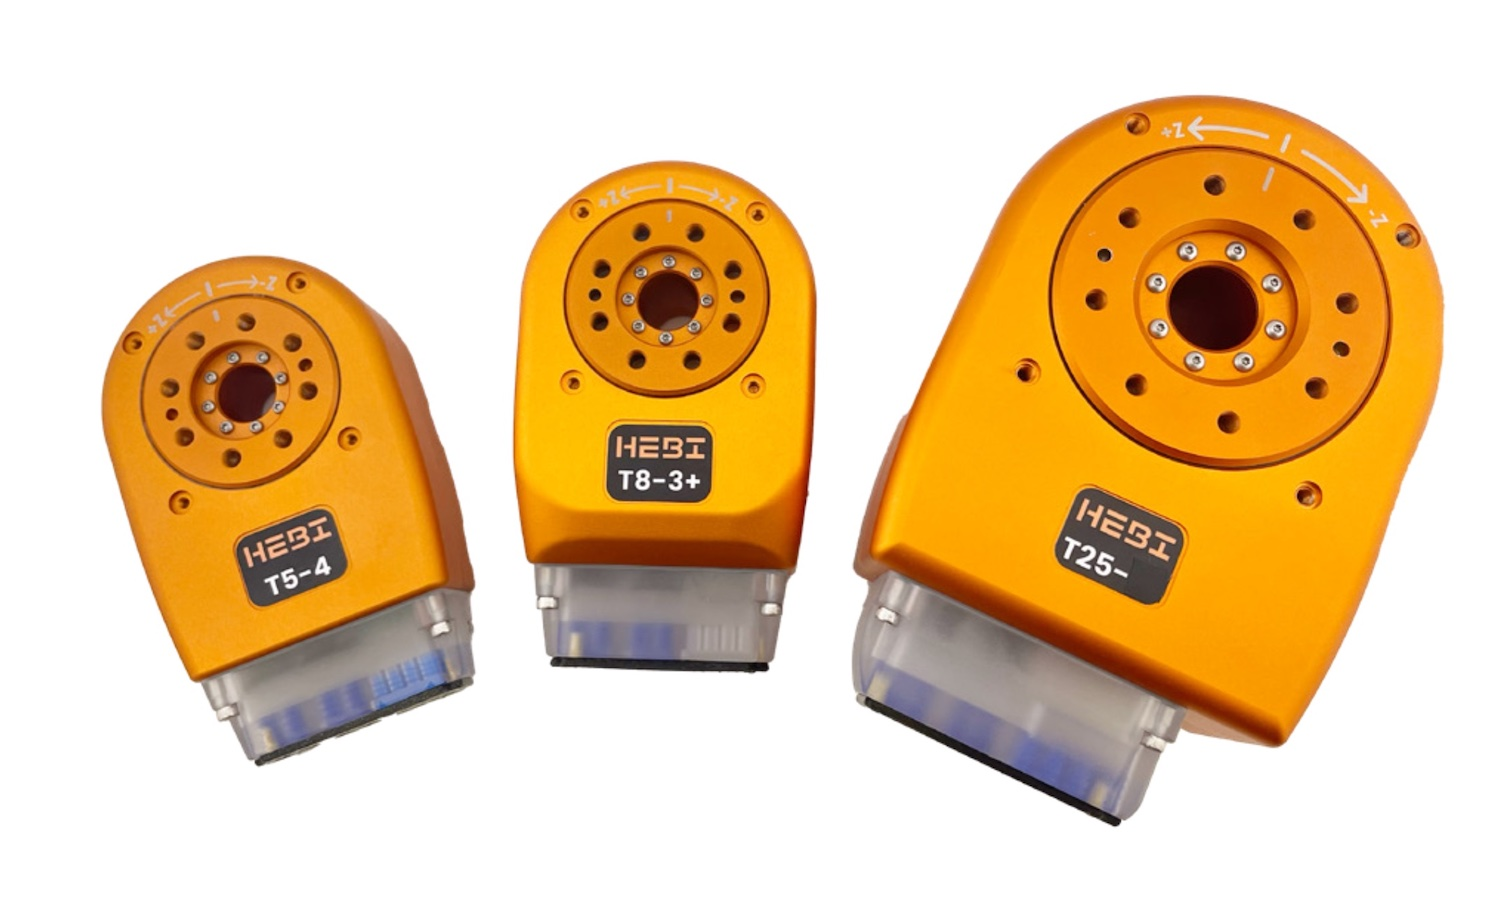
\includegraphics[width=\linewidth]{figs/actuador_T-Series.jpg}
	\end{minipage}
	\caption{Actuador T-Series}
	\label{fig:actuador}
\end{figure}


\chapter{Diseño}
\label{cap:capitulo4}

\begin{flushright}
\begin{minipage}[]{9cm}
\emph{El diseño no es solo lo que se ve y lo que se siente. El diseño es cómo funciona.}\\
\end{minipage}\\

Steve Jobs, \textit{conferencia de lanzamiento del Apple iPod, 2001}\\
\end{flushright}

\vspace{1cm}

Después de definir la plataforma de desarrollo, se procede a explicar el diseño de la aplicación.

El sistema está diseñado para gestionar la rehabilitación motora de pacientes post-ictus mediante la interacción con un brazo robótico.
Esto se lleva a cabo a través de una aplicación que controla diversos parámetros que afectan a la trayectoria, las perturbaciones y nivel de asistencia del brazo.
A continuación, se definen los puntos clave del sistema:
\begin{itemize}
    \item Trayectoria: representa el recorrido deseado que el paciente debe seguir durante la terapia. Es una señal definida por los parámetros de frecuencia, amplitud y tipo de señal (trayecto constante o dinámico). El objetivo es medir la precisión del paciente al seguir la trayectoria.
	\item Perturbación: es una señal que altera la trayectoria. Se define mediante los parámetros de amplitud, duración y tipo (perturbación escalón o sinusoidal). El objetivo es proporcionar un desafío adicional al paciente.
	\item Límites: definen las restricciones físicas de movilidad del brazo robótico. Se establecen un límite inferior (mínimo) y superior (máximo), así como un offset que determina la posición inicial del brazo. Se ajustan llevando el brazo a la posición deseada.
	\item Asistencia: se refiere al grado de apoyo que ofrece el brazo robótico al paciente. Este parámetro se ajusta tanto de forma dinámica, según el nivel de dificultad del juego, como manual, a través de la interfaz de control.
	\item Nivel de dificultad: hace referencia al nivel de dificultad del juego. El nivel de dificultad aumenta de forma progresiva, reduciendo el nivel de asistencia del robot. Puede ajustarse tanto dinámicamente como manualmente al igual que la asistencia.\\
\end{itemize}\

Más adelante, se describen los nodos y topics utilizados en la plataforma.

\section{Esquema de nodos y topics}
\label{section:review}

En la Imagen \ref{fig:nodes} se contempla un esquema de los nodos, topics y tipos de datos que se utilizan para la comunicación de la plataforma software con el actuador.

\begin{figure}[ht!]
	\centering
	\begin{minipage}{1.0\linewidth}
		\centering
		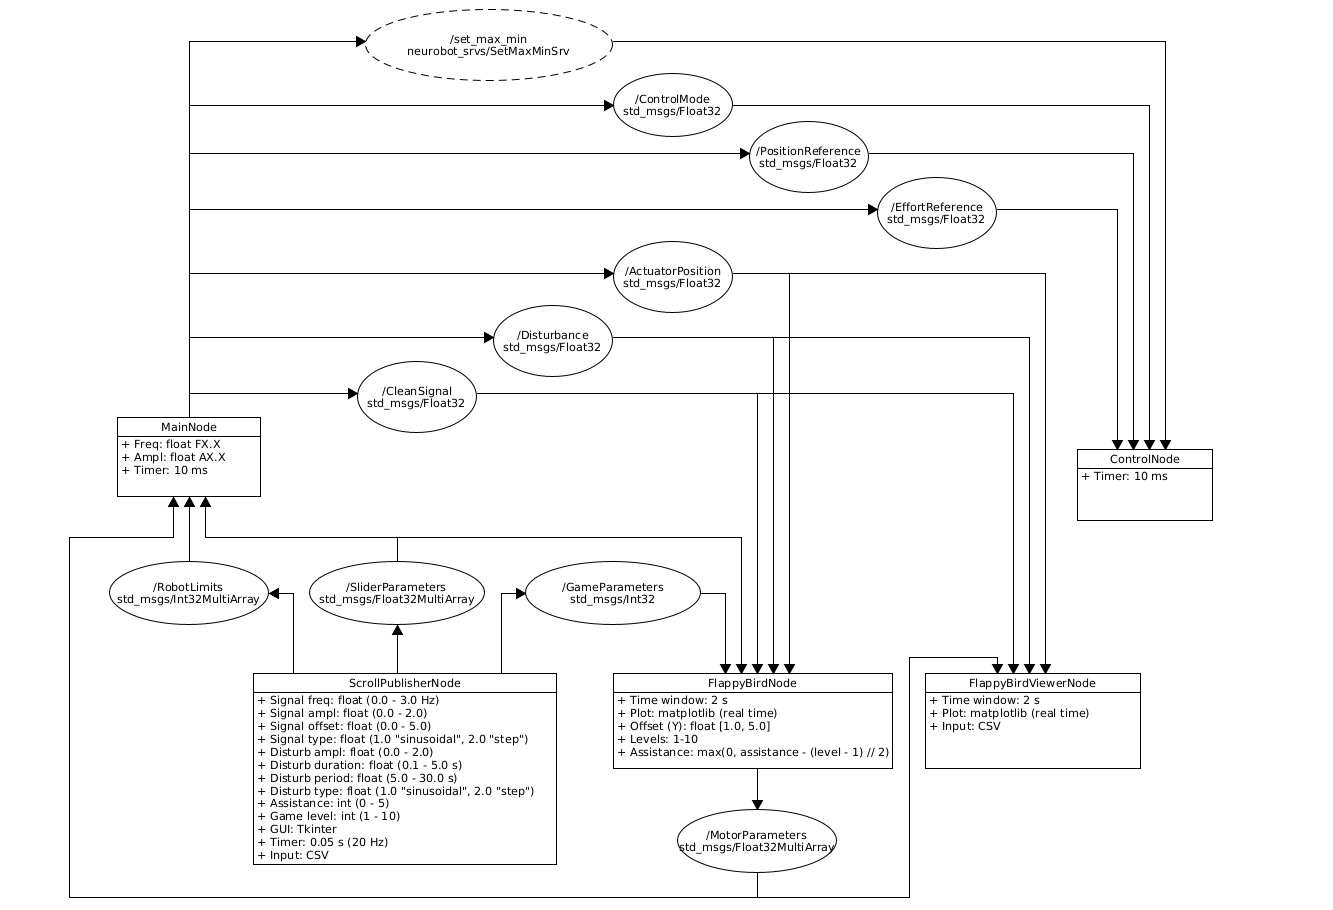
\includegraphics[width=\linewidth]{figs/esquema_nodos.png}
	\end{minipage}
	\caption[Esquema de nodos y topics]{Esquema de nodos y topics}
	\label{fig:nodes}
\end{figure}

Seguidamente, se detalla la función de los nodo y la información trasmitida por cada uno de los topics:
\begin{itemize}
    \item \verb|LimitNode|: este nodo gestiona la configuración de los límites del brazo robótico. Utiliza el topic \verb|/RobotLimits|, como un booleano para indicar el límite que se ajusta.
	\item \verb|ScrollPublisherNode|: este nodo publica los parámetros de la trayectoria y la perturbación en el topic \verb|/SliderParameters|, y del juego (asistencia y nivel de dificultad) en \verb|/GameParameters|. La actualización de los datos se realiza cada $50 ms$.
	\item \verb|FlappyBirdNode|: este nodo implementa la lógica del juego basado en seguir una trayectoria o mantener una posición. Recibe la señal de referencia del topic \verb|/CleanSignal|, la señal de perturbación de \verb|/Disturbance|, la asistencia y nivel de dificultad de \verb|/GameParameters|, los límites y el offset de \verb|/SliderParameters| y la posición del jugador de \verb|/ActuatorPosition|. Y publica los datos de referencia de las señales y tiempo, en el momento de la posición del jugador en el eje X, en el topic \verb|/MotorParameters|. La actualización de los datos se realiza cada $10 ms$.
	\item \verb|FlappyBirdViewerNode|: este nodo grafica las señales de trayectoria, perturbación y la posición del paciente, que recibe de los topics \verb|/CleanSignal|, \verb|/Disturbance| y \verb|/ActuatorPosition|, respectivamente, para visualizar el progreso del paciente durante la terapia. Además, calcula el error de posición a través de los datos publicados en el topic \verb|/MotorParameters|, explicados en el nodo anterior.\\
\end{itemize}\

El proyecto se divide en cuatro scripts, el primero se utiliza para crear o registrar un paciente, el segundo lanza la GUI y controla los parámetros del juego, el tercero permite visualizar el comportamiento del paciente durante la terapia, y el cuarto es el propio juego.

\section{Interfaz de registro de un paciente}
\label{section:registro}

Este script permite gestionar un conjunto de datos, que registran a un paciente, mediante una GUI.

En primer lugar, se importan las bibliotecas estándar, mencionadas en el capítulo anterior, como \verb|tkinter|, que se utiliza para crear la interfaz gráfica, \verb|csv| para guardar los datos en un archivo CSV para su posterior uso, y \verb|os| para interactuar con el sistema de archivos.

Se obtiene el directorio de inicio del usuario y se crea un directorio dentro de este, si no existe, bajo el nombre \textit{database}, donde se almacenan los ficheros con los datos de registro y análisis terapéuticos de cada paciente.

Se definen tres funciones principales que gestionan las operaciones de la GUI.
La función \verb|exit()| cierra la ventana principal de Tkinter, \verb|clear()| limpia los campos de entrada y texto, y \verb|savedata()| guarda los valores de los campos, valida que el ID sea un número y crea un subdirectorio bajo el nombre del ID, si no existe, donde guarda los datos en un archivo CSV llamado \verb|ID.csv|.
Si el archivo no existe, se escribe el encabezado utilizando \verb|writer.writeheader()|.
Los datos se escriben con \verb|csv.DictWriter| y son guardados como \verb|strings|.

Se crea una ventana principal con un título y tamaño fijo de $600x500$ píxeles.
Los estilos visuales se configuran con \verb|ttk.Style| y se definen dos frames distintas, \verb|main_frame| se utiliza como contenedor de los campos de entrada y texto y \verb|button_frame| agrupa la lógica de los botones.
Cada campo es un \verb|Entry| enlazado a una variable de tipo \verb|StringVar| y hacen referencia al nombre, apellido e ID del paciente, frecuencia, amplitud y perturbación de la señal que generará el brazo robótico, nivel y progreso del juego y un espacio para que el doctor incluya observaciones.
Se crean dos botones, \textit{Save} llama a \verb|savedata()| para guardar los datos, que a su vez llama a \verb|clear()| para limpiar los campos una vez que estos se han almacenado, y el botón \textit{Exit} llama a la función \verb|exit()| que cierra la aplicación.
En la Imagen \ref{fig:database} puede observarse el estilo de la interfaz.

\begin{figure}[ht!]
	\centering
	\begin{minipage}{0.65\linewidth}
		\centering
		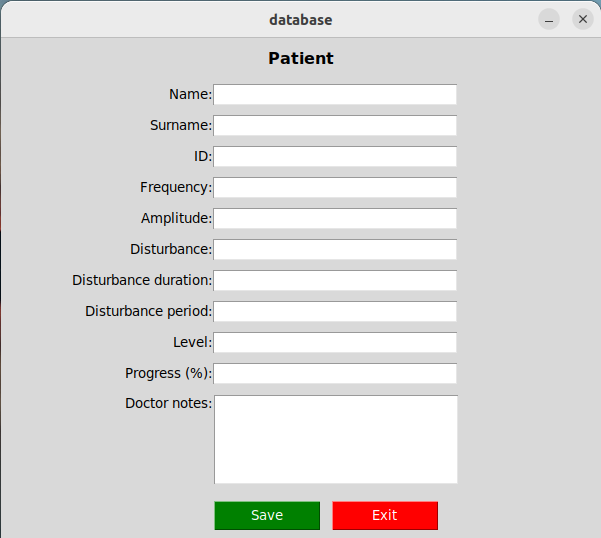
\includegraphics[width=\linewidth]{figs/registro.png}
	\end{minipage}
	\caption[Interfaz de registro de un paciente]{Interfaz de registro de un paciente}
	\label{fig:database}
\end{figure}

\verb|root.mainloop()| inicia el bucle de eventos de Tkinter y la interfaz está activa hasta que el usuario cierra la ventana.

\section{Interfaz de control}
\label{section:controller}

Este script combina ROS 2 y Tkinter para crear una GUI que gestiona límites físicos (mínimo, máximo y offset) del robot, adaptándose al brazo específico del paciente que se va a rehabilitar, configura y publica parámetros para crear una señal de control y perturbación para un sistema robótico, parámetros de asistencia y nivel de dificultad para un videojuego terapéutico y almacena dichas configuraciones por paciente.

Al inicio del script se importan las librerías \verb|rclpy| y \verb|std_msgs.msg| para gestionar la comunicación entre Python y ROS 2, \verb|tkinter| para crear la interfaz gráfica, \verb|csv| para el manejo de archivos CSV, \verb|os| para interactuar con el sistema y \verb|datetime| para gestionar la fecha de creación de los archivos.

Se crea un directorio en el directorio de inicio del usuario, si no existe, bajo el nombre \textit{database}, donde se almacenan los ficheros con los datos de configuración de cada paciente.

Se definen dos clases, \verb|ScrollPublisherNode| y \verb|ScrollGUI|.
La primera es una clase de ROS 2 que publica los parámetros de dos señales, de tipo trayectoria y perturbación en el topic \verb|/SliderParameters| y los datos de asistencia y nivel de juego en \verb|/GameParameters|.
Los mensajes son de tipo \verb|Float32MultiArray| y \verb|Int32MultiArray|, y se publican cada $50 ms$ y únicamente cuando se actualiza el valor de los datos, respectivamente.
La decisión de publicar ambas señales en el mismo topic a dicha velocidad se debe a que la actualización de los datos debe realizarse de forma casi instantánea para permitir ajustes inmediatos en los parámetros de la terapia y evaluar la rapidez de respuesta del paciente.
Y, se ha comprobado que esta estimación es lo suficientemente rápida para satisfacer estos requisitos.
Los datos necesarios para generar la señal de trayectoria son frecuencia, amplitud y tipo, mientras que para la perturbación son duración, amplitud y tipo.
El tiempo de las señales se define de manera distinta para evitar redundancias, ya que la perturbación no es constante.
En su lugar, se estima una duración que facilita el entendimiento del terapeuta.
El tipo de señal hace referencia al modo de juego y se codifica como 1.0 (hold o mantener) y 2.0 (follow o seguir), y el tipo de perturbación como 1.0 (sinusoidal) y 2.0 (step o escalón).
También se define un offset que determina la distancia entre la señal principal y los límites superior e inferior, ajustando así los márgenes del camino.
La segunda clase crea la interfaz gráfica y permite ajustar los parámetros del juego en tiempo real y publicarlos a través de un nodo de ROS.
Los datos se guardan en un archivo CSV bajo el nombre \verb|ID-year-month-day-config_<index>.csv| en un subdirectorio llamado \textit{config} dentro del directorio \textit{home/user/database/ID/}.
\verb|index| hace referencia al número de archivo de la sesión diaria.
Si el archivo no existe, se escribe un encabezado con los nombres de los campos a los que hacen referencia los datos como se observa en el Código \ref{cod:codejemplo2}.

\begin{code}[h]
\begin{lstlisting}[language=Python]
header = ["frequency", "amplitude", "offset", "signal", "disturbance", "duration", "period", "mode"]
\end{lstlisting}
\caption[Encabezado del fichero de configuración]{Encabezado del fichero de configuración}
\label{cod:codejemplo2}
\end{code}

Se crean deslizadores, utilizando \verb|ttk.Scale|, para ajustar la frecuencia, amplitud, offset, duración y periodo de las señales, lo que facilita la configuración de los parámetros con mayor precisión y comodidad.
Se utiliza \verb|Combox| para permitir la selección entre los distintos tipos de señal y perturbación y niveles de asistencia (del 0 al 5, donde 0 es asistencia nula y 5 asistencia máxima) y de juego (del 1 al 10, de menor a mayor dificultad).
Los botones \textit{Update Signal} y \textit{Update levels} se utilizan para actualizar los datos en el topic correspondiente, y el botón \textit{Exit} para salir.
En la Imagen \ref{fig:control} se observa el aspecto de la ventana principal de control.

\begin{figure}[ht!]
	\centering
	\begin{minipage}{0.55\linewidth}
		\centering
		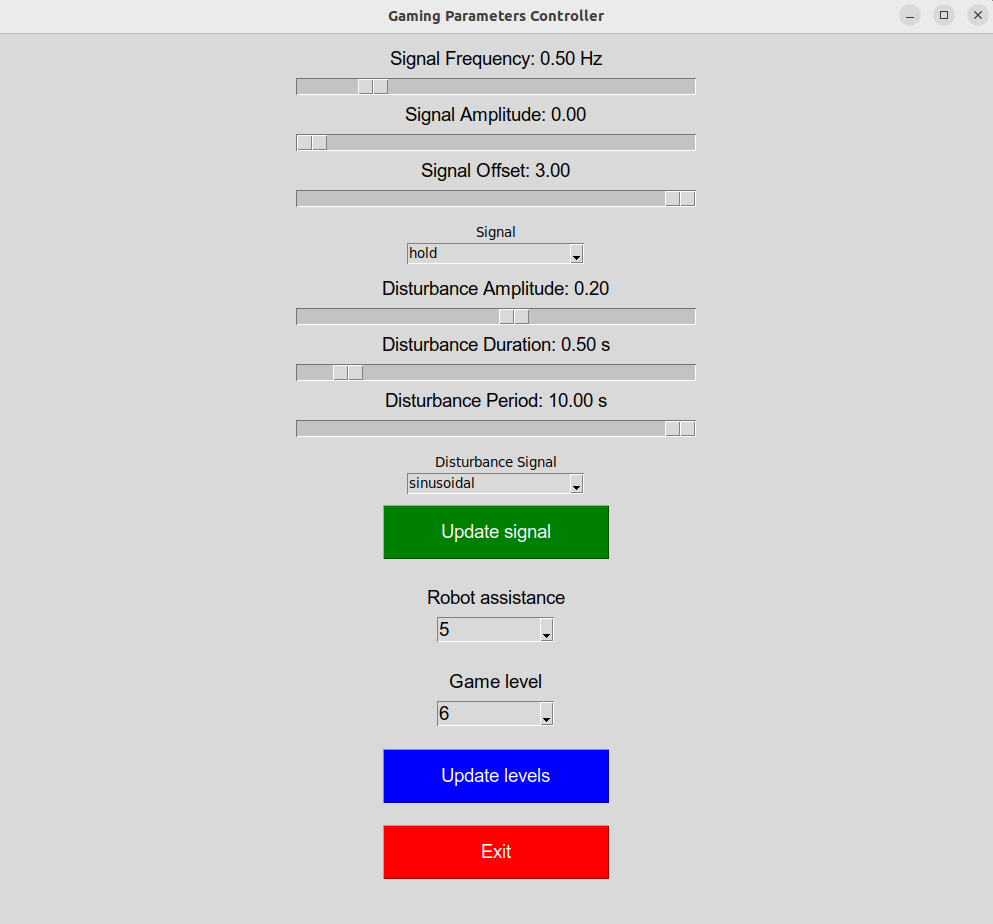
\includegraphics[width=\linewidth]{figs/control_pannel.png}
	\end{minipage}
	\caption[Interfaz de configuración de los parámetros terapéuticos]{Interfaz de configuración de los parámetros terapéuticos}
	\label{fig:control}
\end{figure}

La función \verb|saveconfig()| guarda la configuración actual de la GUI en el archivo CSV.
Las funciones \verb|update*()| convierten el valor del deslizador de \verb|str| a \verb|float|.
Entre ellas se destacan \verb|updatesignal()|, que actualiza los atributos del nodo y llama a \verb|saveconfig()|, que añade al final del archivo la nueva configuración, y \verb|updatelevel()|, que publica un mensaje con los datos de asistencia y nivel de dificultad del juego.
La función \verb|close()| finaliza el nodo y cierra la GUI y el método \verb|run()| inicia el bucle de eventos de Tkinter junto con \verb|spin_once()|.
\verb|loadcsv()| lee el último registro del archivo del paciente que se pasa como parámetro y devuelve los valores de frecuencia (Hz), amplitud (rad) de las señales de trayectoria y perturbación, duración (s), periodo (s) y nivel del juego.
Todos son \verb|float| excepto el último que es un \verb|int|.

\verb|main()| es la función principal y se encarga de extraer el ID del paciente desde la ruta al archivo de registro, cargar los datos de las señales y el juego desde el CSV, crear el nodo \verb|ScrollPublisherNode| con dichos parámetros e iniciar la GUI.
\verb|startgui()| es la primera interfaz que se lanza y gestiona la configuración del brazo que se va a rehabilitar y de los límites físicos del robot a través de la publicación de un \verb|Int32MultiArray| que actúa como un booleano indicando el botón que se ha pulsado (resetear, mínimo, máximo u offset).
El offset corresponde a la posición inicial desde la cual comienza la terapia.
Además, comprueba que se ha seleccionado o bien brazo derecho o izquierdo y que los límites mínimo y máximo se han definido correctamente antes de permitir establecer el offset o continuar a la siguiente ventana.
La decisión de ajustar los límites y el offset mediante el movimiento del brazo robótico a una posición específica, y luego guardar dicha posición a través de un botón, responde a un requisito explícito del cliente.
En la Imagen \ref{fig:config} se muestra el formato de la ventana de inicio.

\begin{figure}[ht!]
	\centering
	\begin{minipage}{0.45\linewidth}
		\centering
		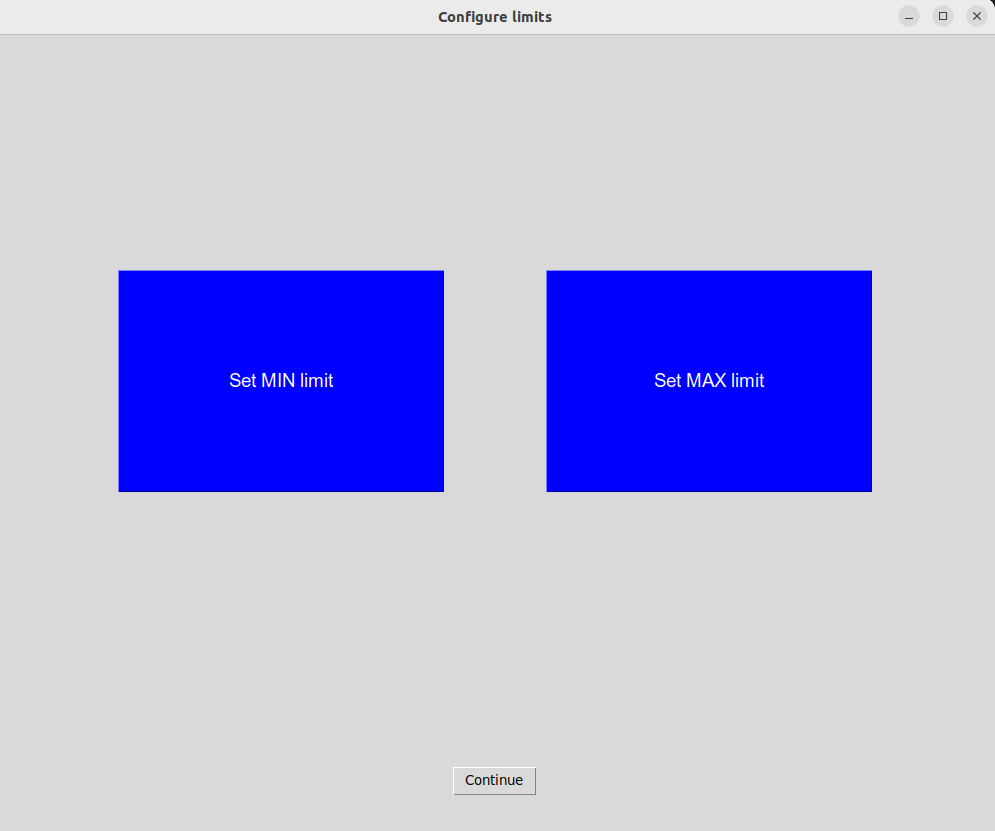
\includegraphics[width=\linewidth]{figs/config_limits.png}
	\end{minipage}
	\caption[Interfaz de configuración de los límites y orientación del brazo robótico]{Interfaz de configuración de los límites y orientación del brazo robótico}
	\label{fig:config}
\end{figure}

\section{Interfaz de visualización}
\label{section:visualization}

Este script permite observar y registrar la ejecución de un paciente en una tarea de seguimiento de trayectoria como parte de una sesión de rehabilitación motora.

Además de incluir las bibliotecas mencionadas en la Sección \ref{section:controller}, se utilizan \verb|matplotlib| para visualizar los datos del rendimiento del jugador en tiempo real, \verb|numpy| para manejar los datos de las señales que cambian con el tiempo y \verb|sys| para gestionar la ruta al archivo CSV con los datos de registro del paciente.

Se utiliza el modo interactivo de \verb|matplotlib|, \verb|plt.ion()|, que permite actualizar dinámicamente los gráficos sin bloquear el hilo principal.
Las ventanas son deslizantes respecto al eje X, no obstante debemos mantener un tamaño fijo para que la señal no se desplace hacia la izquierda, por ello se implementa \verb|np.roll()|.
El tamaño de la ventana en el eje Y se ajusta a $3$ ya que es el máximo recorrido que puede hacer el brazo.

Se define la clase \verb|FlappyBirdViewerNode| que actúa como nodo de ROS 2 y se suscribe a los topics \verb|/CleanSignal|, donde se publica la señal de referencia que se toma como trayectoria deseada que el jugador debe seguir, \verb|/Disturbance|, que contiene la señal de perturbación, \verb|/ActuatorPosition|, que publica la posición del jugador en el eje Y, y \verb|/MotorParameters|, para obtener el tiempo del juego, la posición del jugador en el eje X y el nivel de asistencia del robot.
Los mensajes de los primeros tres topics son de tipo \verb|Float32| y el último es un \verb|Float32MultiArray|.
\verb|signalcallback()| se activa cada vez que se recibe un valor de la señal, si el jugador está activo se actualizan los datos (tiempo, límites, posición, error de trayectoria y detección de colisiones) y se grafican.
Para la detección de colisiones se implementa una lógica simple basada en la comparación de la posición del jugador con los límites de la señal.
\verb|playercallback()| actualiza la posición del jugador, el offset que separa la señal de los límites y el tiempo total y marca que el jugador está activo.

En la Imagen \ref{fig:visual}, se muestran dos gráficos.
El que está en la parte superior muestra la señal de trayectoria (línea azul), la perturbación de tipo escalón (línea verde), los límites superior e inferior (líneas discontinuas grises) y la posición actual del jugador (punto rojo), proporcionando una visión clara y completa de la terapia.
Y, la parte inferior grafica el error de posición con respecto a la trayectoria deseada en función del tiempo, lo que permite detectar fallos de control, fatiga o pérdida de atención.

\begin{figure}[ht!]
	\centering
	\begin{minipage}{0.80\linewidth}
		\centering
		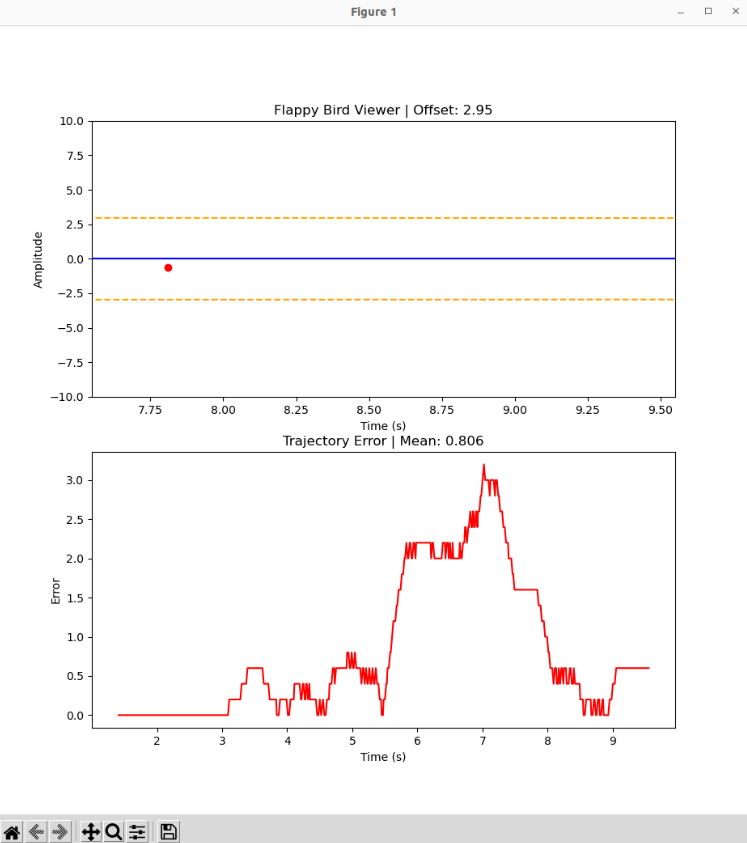
\includegraphics[width=\linewidth]{figs/visual.png}
	\end{minipage}
	\caption[Interfaz de visualización del terapeuta]{Interfaz de visualización del terapeuta}
	\label{fig:visual}
\end{figure}

En un principio, el error se calculaba en función del tiempo como se muestra en la Ecuación \ref{ec:ec1}, pero, más adelante, se optó por calcular la interpolación (o selección por índice más cercano) del valor de la trayectoria de referencia (x, y) evaluando la posición del jugador en el eje X, $x_p$, como se muestra en la Ecuación \ref{ec:ec2}.
El segundo cálculo ofrece una aproximación más precisa al error, ya que está directamente relacionado con la ubicación del jugador.
A diferencia del primer cálculo, que depende del instante de tiempo y puede verse afectado por variaciones en la sincronización de los datos.

\begin{myequation}[h]
\begin{equation}
error_t = | y_{player}(t) - y_{reference}(t) |
\nonumber
\label{ec:ec1}
\end{equation}
\caption[Cálculo del error de trayectoria en el tiempo]{Cálculo del error de trayectoria en el tiempo}

\begin{equation}
error(x_p, y_p) = | y_p - f(x_p) |
\nonumber
\label{ec:ec2}
\end{equation}
\caption[Cálculo del error de trayectoria por posición]{Cálculo del error de trayectoria por posición}
\end{myequation}

Al finalizar la ejecución, los datos más relevantes como el tiempo, la señal, los límites mínimo y máximo, la posición del jugador, el offset, el error, las colisiones y el nivel de asistencia se almacenan en un archivo CSV bajo el nombre \verb|ID-year-month-day-metrics_<index>.csv| en un subdirectorio llamado \textit{metrics} dentro del directorio \textit{home/user/database/ID/}.
\verb|index| hace referencia al número de archivo de la sesión diaria.
Esto facilita un análisis posterior de la terapia.

La función principal \verb|main()| verifica que se ha pasado como único argumento un archivo CSV con los datos de registro del paciente, extrae el ID desde la ruta, crea el nodo \verb|FlappyBirdViewerNode| y escucha de los topics.

\section{Juego flappy}
\label{section:game}

Este script implementa un juego basado en el Flappy Bird, adaptado a un entorno ROS 2 para interactuar con sensores y actuadores en tiempo real.
Existen dos modos de juego distintos, \textit{hold}, el jugador debe mantener la posición, y \textit{follow}, el jugador debe seguir una trayectoría.

Se implementan las librerías \verb|rclpy|, y \verb|std_msgs| para permitir la comunicación con ROS 2, \verb|matplotlib| y \verb|numpy| para la visualización y el manejo de señales, y \verb|pygame| para utilizar efectos de sonido.

Se emplean sonidos distintos cuando se sube de nivel, se consigue una recompensa o se colisiona.
Esto permite que el juego sea más interactivo.
En el Código \ref{cod:codejemplo3}, escrito en \textit{Python}, se observa como se carga un sonido desde un directorio, \textit{sounds}, dentro del paquete del proyecto.
Los formatos de audio más comunes soportados por \verb|pygame.mixer| son .wav, .ogg y .mp3.
La elección de utilizar la extensión .wav se debe a su simplicidad, alta calidad y compatibilidad con todos los sistemas.

\begin{code}[h]
\begin{lstlisting}[language=Python]
pygame.mixer.init()
level_up_sound = pygame.mixer.Sound('../sounds/level_up.wav')
\end{lstlisting}
\caption[Cargar un sonido al juego]{Cargar un sonido al juego}
\label{cod:codejemplo3}
\end{code}

La clase \verb|FlappyBirdNode| engloba la lógica del programa.
En \verb|__init__| se crean los suscriptores \verb|/CleanSignal|, de tipo \verb|Float32|, es la señal de referencia, \verb|/Disturbance|, también \verb|Float32|, es la perturbación, \verb|/GameParameters|, es un \verb|Int32MultiArray|, contiene el nivel del juego y de asistencia del robot, \verb|/SliderParameters|, \verb|Float32MultiArray|, para obtener el offset entre la señal y los límites superior e inferior, y \verb|/ActuatorPosition|, es un \verb|Float32|, contiene la posición del jugador en el eje Y.
Se crea un publicador \verb|Float32MultiArray|, llamado \verb|/MotorParameters|, que contiene la marca de tiempo de la ventana, las referencias de la señal y la perturbación en $(x_p, y)$, la posición del jugador en el eje X y la asistencia actualizada.
Se crea una ventana gráfica de tamaño $2x3$, donde 3 es el recorrido máximo del brazo.
En ella se representan la señal principal, los límites mínimo y máximo, las perturbaciones, la posición del jugador y objetos como estrellas y asteroides que forman parte de la lógica del juego.

La posición del jugador se representa como un punto rojo que cambia de color según la distancia a la que se encuentra entre la trayectoria deseada y los límites (negro significa que está cerca de la trayectoria, gris que está a una distancia media y rojo indica peligro de colisión con los límites).
La posición se representa como una coordenada en los ejes XY, en el eje X permanece siempre a la misma distancia (a $0,25$ unidades del origen), y en el eje Y se muestra la posición que se recibe del sensor de posición del motor.
En un principio, para validar el movimiento del jugador, la posición en el eje Y se basaba en el manejo de las flechas arriba y abajo del teclado.
Para ello se utilizó la librería \verb|pynput|.
En el Código \ref{cod:codejemplo4}, escrito en Python, se muestra la lógica de las teclas.

\begin{code}[h]
\begin{lstlisting}[language=Python]
def on_press(self, key):
	try:
		direction = -1 if self.inverted_gravity else 1
		if key == keyboard.Key.up:
			self.player_y += 0.1 * direction
		elif key == keyboard.Key.down:
			self.player_y -= 0.1 * direction
	except:
		pass
\end{lstlisting}
\caption[Movimiento vertical del jugador]{Movimiento vertical del jugador}
\label{cod:codejemplo4}
\end{code}

El método \verb|updatelevel()| cambia los colores del fondo y de la línea según el nivel, reproduce el sonido de subida de nivel y disminuye la asistencia para que la dificultad sea progresiva.
La asistencia del robot se disminuye utilizando la Fórmula \ref{ec:ec3}.
Se utiliza el máximo entre 0 y el valor calculado según el nivel para que la asistencia no sea un valor negativo.

\begin{myequation}[h]
\begin{equation}
assistance = max(0, assistance - (level - 1) // 2)
\nonumber
\label{ec:ec3}
\end{equation}
\caption[Cálculo del nivel de asistencia según el nivel de dificultad]{Cálculo del nivel de asistencia según el nivel de dificultad}
\end{myequation}

Para crear un juego dinámico que capte la atención del paciente se crea una misión secundaria en cada nivel.
Los niveles 1, 4 y 7 tienen como objetivo permanecer dentro de los límites por un tiempo determinado.
Esto permite evaluar la precisión del paciente.
Además, cuando se sobrepasa uno de los límites el contador se para y se reanuda de nuevo cuando se vuelve al camino.
Los niveles 2 y 6 se enfocan en el ajuste de la posición para chocar con las estrellas que están dispuestas en la señal principal.
De esta forma se consigue que el paciente permanezca y siga la trayectoria deseada.
Los niveles 3 y 8 pretenden ejercitar la rapidez de reacción mientras el paciente evita colisionar con los asteroides.
Los niveles 5 y 9 fomentan la flexibilidad cognitiva del paciente para adaptarse a una nueva lógica de control basada en el concepto de gravedad invertida (arriba es abajo y viceversa).
Y, por último, el nivel 10 permite al médico evaluar distintos escenarios límites mediante ajustes en los parámetros de la señal, perturbación y el offset.
En las Imágenes \ref{fig:level} y \ref{fig:level2} se comparan dos niveles diferentes del juego.
La primera imagen presenta límites más estrictos que la segunda, que se han coloreado para que se vean claramente en el estudio, pero en el juego son dos líneas de color blanco punteadas para evitar distracciones del paciente.
En la segunda imagen, se observan dos perturbaciones de tipo sinusoidal con sentidos opuestos, representadas por triángulos verdes cuya punta indica el signo de la perturbación.
Si fuese una perturbación de tipo escalón, los triángulos se pintan de color naranja siguiendo la misma lógica de graficación.
En contraste, la primera imagen no muestra ninguna perturbación.

\begin{figure}[ht!]
	\centering
	\begin{minipage}{0.85\linewidth}
		\centering
		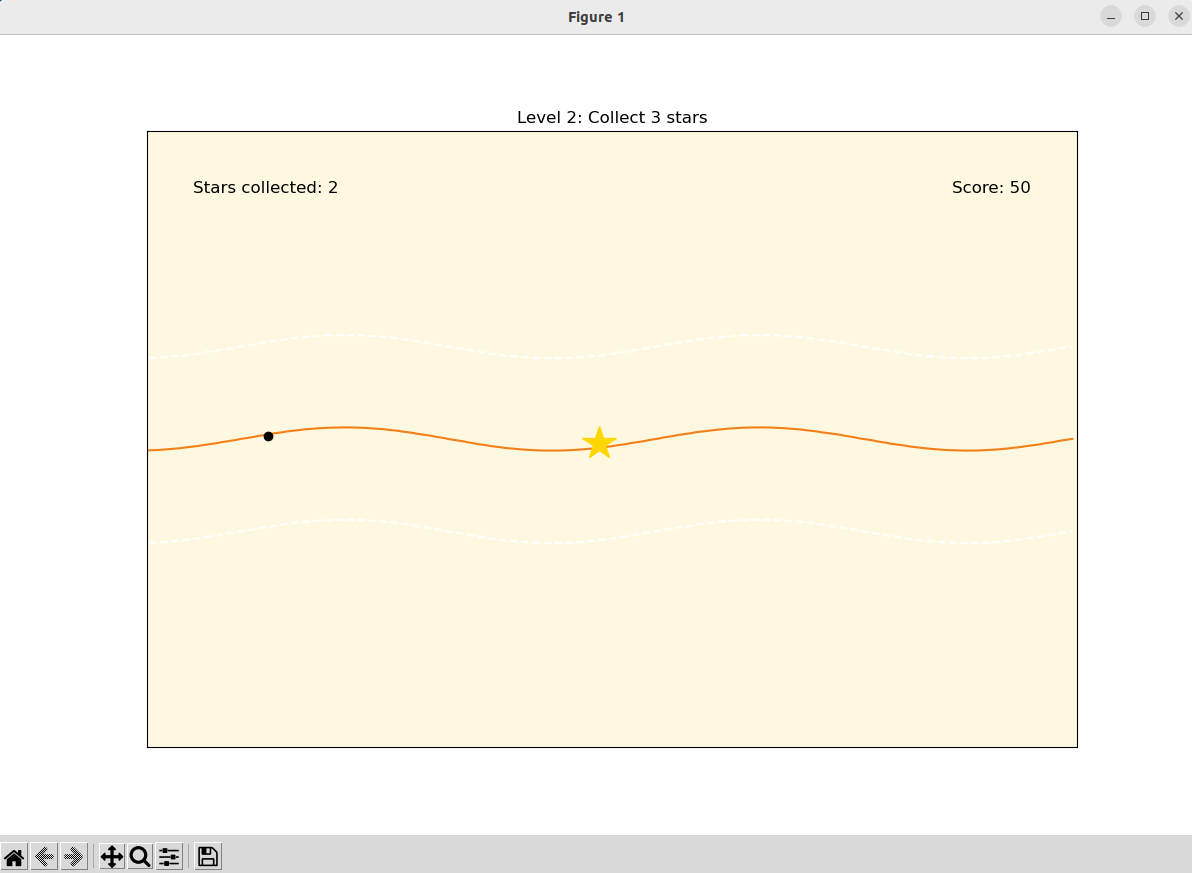
\includegraphics[width=\linewidth]{figs/flappy_level.png}
	\end{minipage}
	\caption[Nivel 2 del juego sin perturbación]{Nivel 2 del juego sin perturbación}
	\label{fig:level}
\end{figure}

\begin{figure}[ht!]
	\centering
	\begin{minipage}{0.70\linewidth}
		\centering
		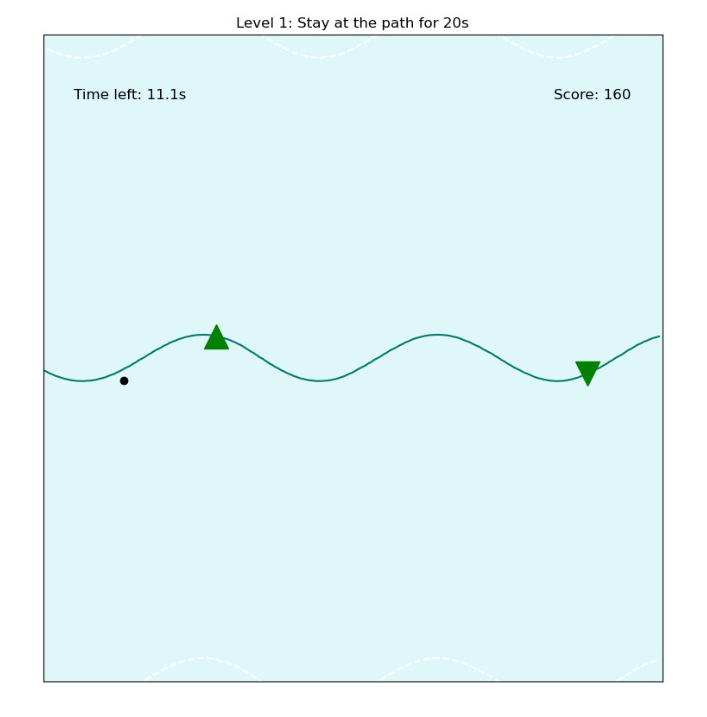
\includegraphics[width=\linewidth]{figs/flappy_level2.png}
	\end{minipage}
	\caption[Nivel 1 del juego con perturbación]{Nivel 1 del juego con perturbación}
	\label{fig:level2}
\end{figure}

Se introduce un sistema de recompensas para aumentar la motivación y destreza del paciente.
Esto permite reforzar comportamientos y habilidades específicas para alcanzar los objetivos propuestos.
Cada vez que se consigue una estrella y se sube de nivel se suman 10 y 30 puntos, respectivamente, a un contador.
Y, cuando se colisiona con un asteroide, el contador decrementa en 5 puntos.
Para ello se utilizan las funciones \verb|incrementscore()| y \verb|decrementscore()|.

Los objetos como las estrellas, los asteroides y los triángulos, que indican el sentido y comienzo de una perturbación, se crean con \verb|ax.plot|.
Las estrellas se generan de forma aleatoria en el eje X, y los asteroides en ambos ejes con límites definidos entre $(0.3, offset)$ y $(-offset, -0.3)$.
El máximo de objetos visuales al mismo tiempo dentro de la ventana es 2.
Las funciones \verb|generatestar()|, \verb|generateasteroid()| y \verb|generatedisturb()| encapsulan la lógica de creación de objetos, y la función \verb|clearobjects()| la eliminación de estos.

El desarrollo del juego está concentrado en \verb|listenercallback()|, que es el bucle principal y se ejecuta cada vez que se recibe un nuevo dato en el topic \verb|/CleanSignal|.
Se utilizan las funciones \verb|np.roll| y \verb|plt.ion()| de las bibliotecas \verb|NumPy| y \verb|Matplotlib|, respectivamente.
\verb|np.roll| actualiza la señal y la perturbación.
Como se explica en la Sección \ref{section:visualization}, los gráficos se actualizan en tiempo real con \verb|plt.ion()|.

Los callbacks actualizan los datos que se reciben de los topics, estas funciones son \verb|disturbcallback()|, \verb|levelcallback()|, \verb|offsetcallback()| y \verb|positioncallback()|.

La función \verb|main()| inicializa el nodo ROS, crea una instancia del juego y entra en un bucle hasta que el usuario detenga el programa.\\

El proyecto es fácilmente escalable en el caso que se quiera añadir una señal que sea combinación de otras.
Simplemente se debe obtener la señal del topic \verb|/CleanSignal| si es de tipo trayectoria o de \verb|/Disturbance| si es de tipo perturbación.
En cuanto a la selección de esta nueva señal, es suficiente con incluir una nueva opción dentro de la \verb|Combox| a la que hace referencia.


\chapter{Resultados y validación}
\label{cap:capitulo5}

\vspace{1cm}

Una vez finalizado el desarrollo del proyecto, se evalúa la usabilidad de la plataforma mediante una encuesta de satisfacción a los usuarios, quienes valoraron su funcionamiento.\\

Se ha realizado una encuesta con 9 preguntas sobre la experiencia del juego a personas sanas.
Los resultados obtenidos han sido los siguientes (n=9):
\begin{figure}[ht!]
	\centering
	\begin{minipage}{0.75\linewidth}
		\centering
		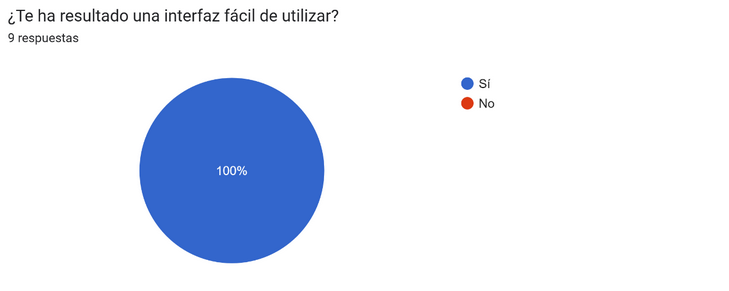
\includegraphics[width=\linewidth]{figs/pregunta1.png}
	\end{minipage}
	\caption[Encuesta de satisfacción. Pregunta 1]{El $100\%$ de los participantes considera que la interfaz es sencilla}
	\label{fig:level1}
\end{figure}

\begin{figure}[ht!]
	\centering
	\begin{minipage}{0.75\linewidth}
		\centering
		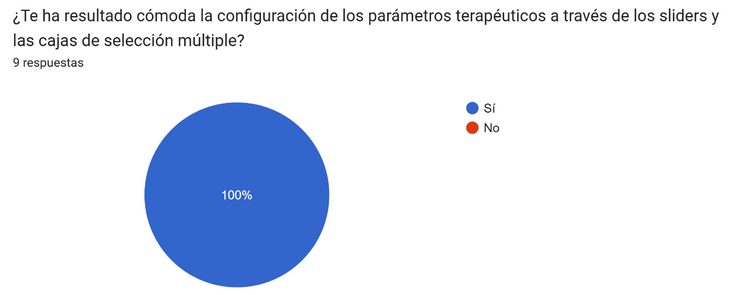
\includegraphics[width=\linewidth]{figs/pregunta2.png}
	\end{minipage}
	\caption[Encuesta de satisfacción. Pregunta 2]{El $100\%$ de los participantes está de acuerdo con que el diseño de la interfaz de control es cómoda de utilizar}
	\label{fig:level2}
\end{figure}

\begin{figure}[ht!]
	\centering
	\begin{minipage}{0.75\linewidth}
		\centering
		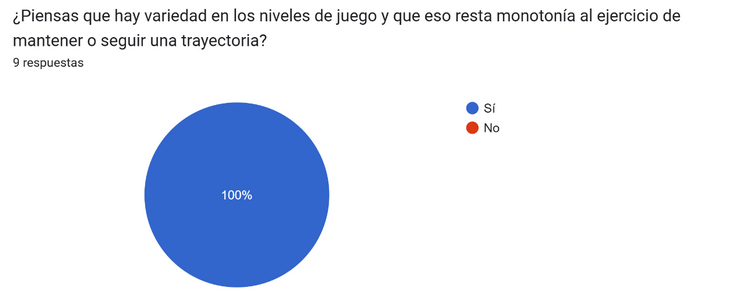
\includegraphics[width=\linewidth]{figs/pregunta3.png}
	\end{minipage}
	\caption[Encuesta de satisfacción. Pregunta 3]{El $100\%$ de los participantes ha votado que hay variedad en los niveles de juego}
	\label{fig:level3}
\end{figure}

\begin{figure}[ht!]
	\centering
	\begin{minipage}{0.71\linewidth}
		\centering
		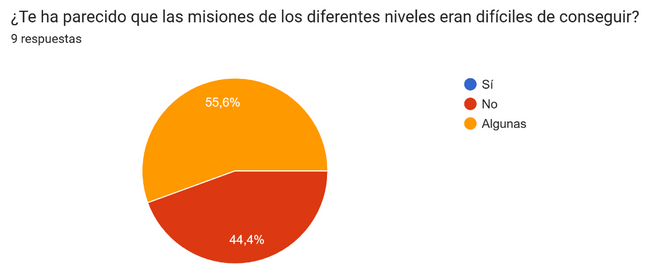
\includegraphics[width=\linewidth]{figs/pregunta4.png}
	\end{minipage}
	\caption[Encuesta de satisfacción. Pregunta 4]{El $55,6\%$ de los participantes piensa que algunas misiones del juego son difíciles de superar y el $44,4\%$ no cree que sean complejas}
	\label{fig:level1}
\end{figure}

\begin{figure}[ht!]
	\centering
	\begin{minipage}{0.85\linewidth}
		\centering
		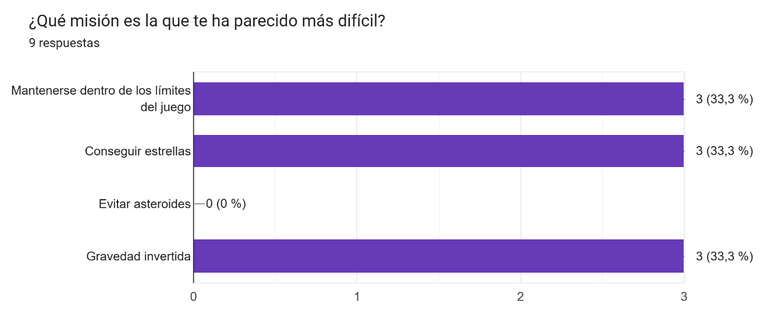
\includegraphics[width=\linewidth]{figs/pregunta5.png}
	\end{minipage}
	\caption[Encuesta de satisfacción. Pregunta 5]{Las misiones más difíciles según los usuarios son: mantenerse dentro de los límites del juego, conseguir estrellas y gravedad invertida}
	\label{fig:level2}
\end{figure}

\begin{figure}[ht!]
	\centering
	\begin{minipage}{0.85\linewidth}
		\centering
		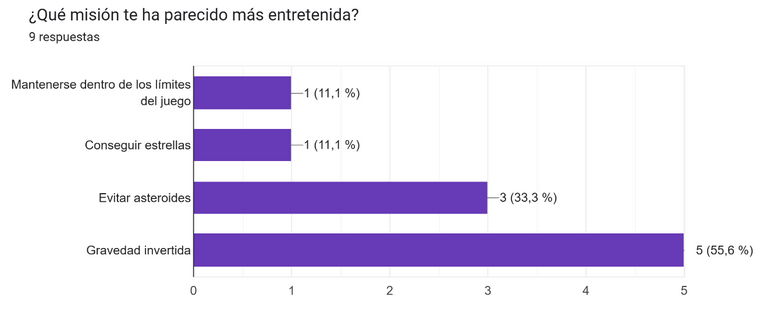
\includegraphics[width=\linewidth]{figs/pregunta6.png}
	\end{minipage}
	\caption[Encuesta de satisfacción. Pregunta 6]{El $55,6\%$ de los participantes ha votado que la misión más entretenida es la de gravedad invertida}
	\label{fig:level3}
\end{figure}

\begin{figure}[ht!]
	\centering
	\begin{minipage}{0.75\linewidth}
		\centering
		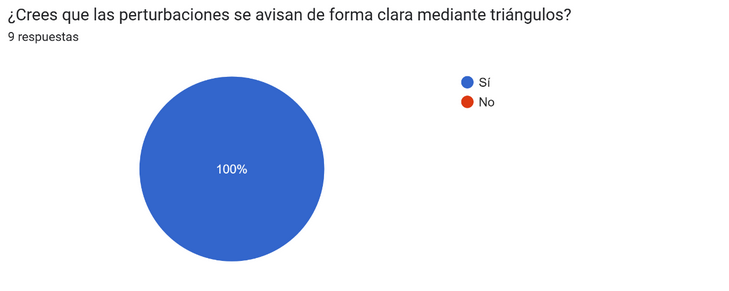
\includegraphics[width=\linewidth]{figs/pregunta7.png}
	\end{minipage}
	\caption[Encuesta de satisfacción. Pregunta 7]{El $100\%$ de los participantes piensa que las perturbaciones están bien señalizadas en el juego}
	\label{fig:level1}
\end{figure}

\begin{figure}[ht!]
	\centering
	\begin{minipage}{0.75\linewidth}
		\centering
		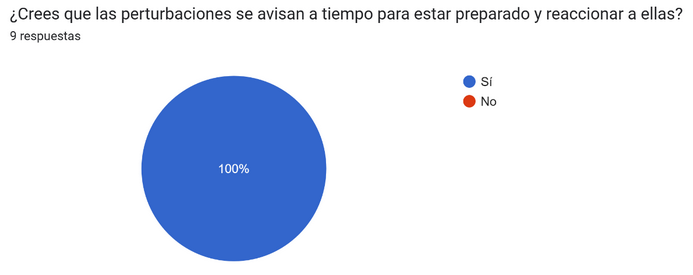
\includegraphics[width=\linewidth]{figs/pregunta8.png}
	\end{minipage}
	\caption[Encuesta de satisfacción. Pregunta 8]{El $100\%$ de los participantes considera que las perturbaciones aparecen con anterioridad antes de que sean notables}
	\label{fig:level2}
\end{figure}

\begin{figure}[ht!]
	\centering
	\begin{minipage}{0.85\linewidth}
		\centering
		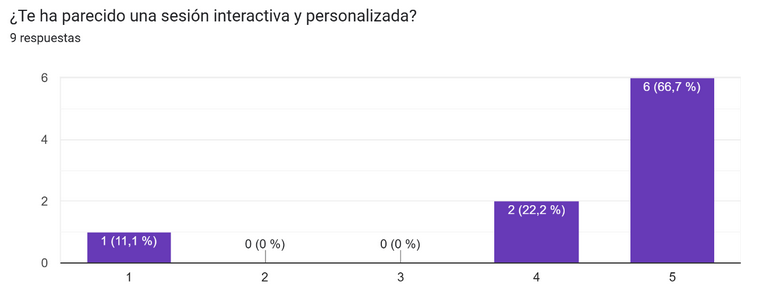
\includegraphics[width=\linewidth]{figs/pregunta9.png}
	\end{minipage}
	\caption[Encuesta de satisfacción. Pregunta 9]{El $66,7\%$ de los participantes ha votado que la sesión terapéutica es interactiva y personalizada}
	\label{fig:level3}
\end{figure}

Como conclusión se refleja que la interfaz del juego es sencilla (el $100\%$ de los participantes así lo consideran), que unas misiones son más entretenidas y difíciles que otras y que las sesiones son interactivas y personalizadas (el $66,7\%$ de los participantes en la encuesta han contestado la mayor puntuación).

Está pendiente realizar la encuesta con pacientes post-ictus.


\clearpage
\thispagestyle{empty}

\printindex \nocite{*}
\appendix
\bibliographystyle{apalike} \bibliography{bibliografia}

\end{document}
